\chapter{Tvorba grafických komponentov v Inkscape}

Vytvorenie SVG v programe Inkscape .


\begin{figure}[ht]
	\begin{center}
		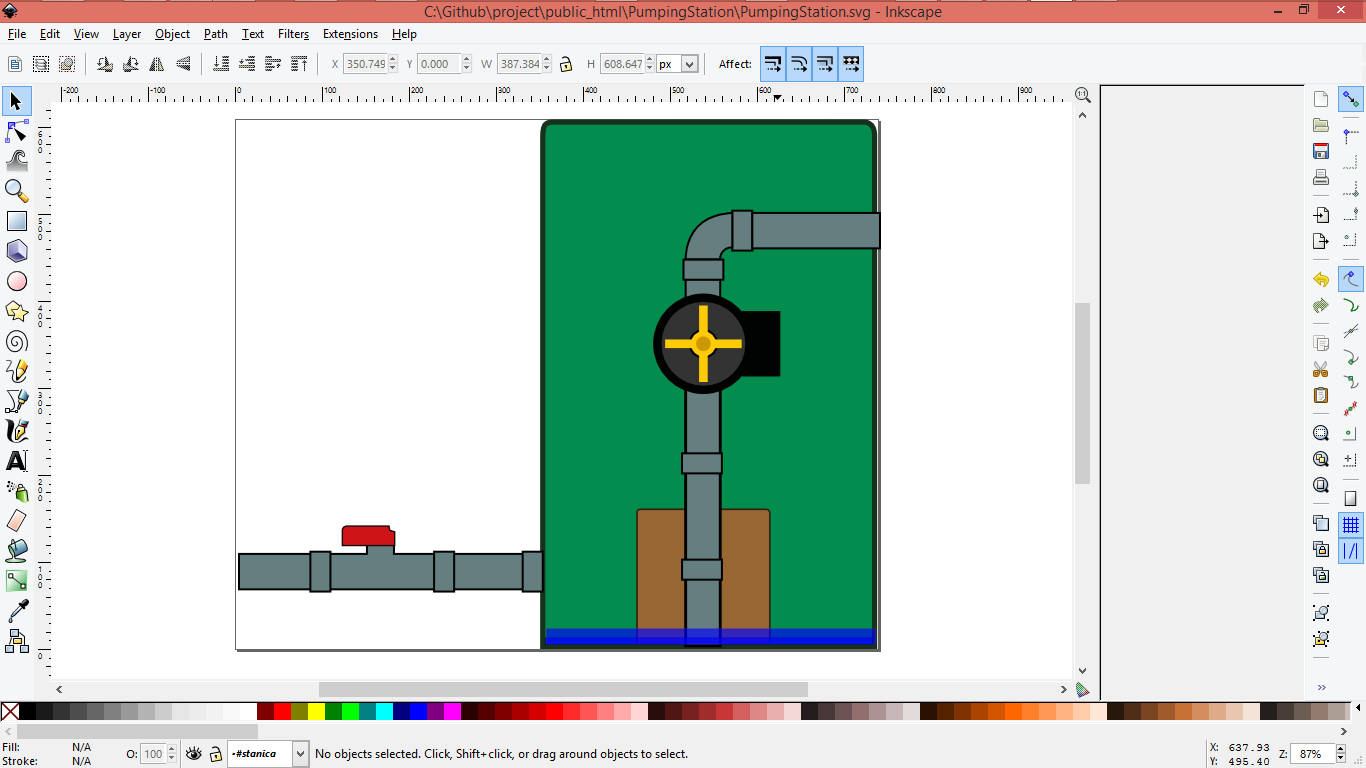
\includegraphics [width=12.5cm] {obrazky/obr1.png}
		\caption{obrázok 1}
		\label{picture1}
	\end{center}
\end{figure}

Nakreslenie jednotlivých častí komponentov pomocou bočného panela. 

Pre ovládanie JavaScriptom je nutné si pozrieť jednotlivé ID SVG Klikneme pravým tlačidlom na daný komponent, časť, a potom na Objekt Properties.

\begin{figure}[ht]
	\begin{center}
		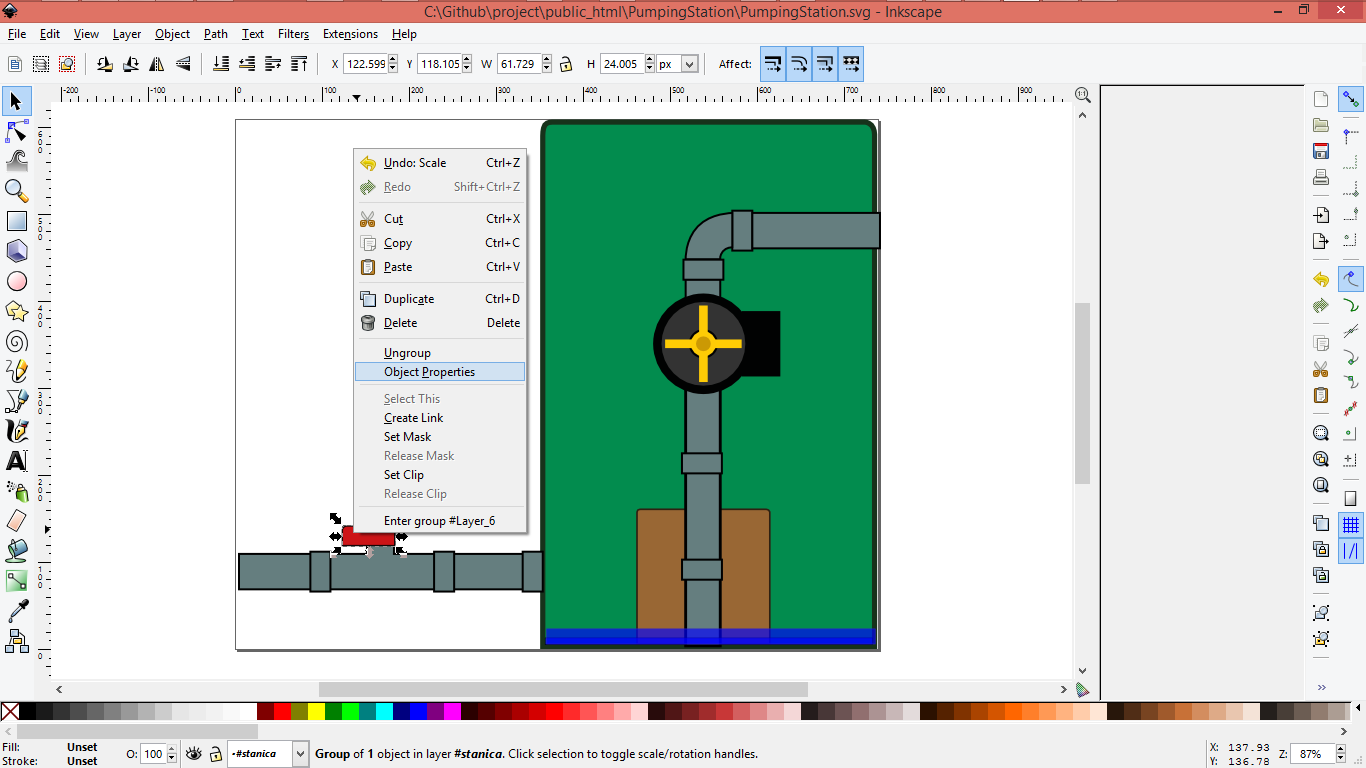
\includegraphics [width=12.5cm] {obrazky/obr2.png}
		\caption{obrázok 2}
		\label{picture2}
	\end{center}
\end{figure}

Zobrazí sa nám nasledovné okno obrázok č.x. 

\begin{figure}[ht]
	\begin{center}
		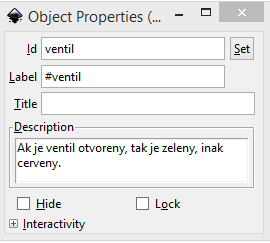
\includegraphics  {obrazky/obr3.png}
		\caption{obrázok 3}
		\label{picture3}
	\end{center}
\end{figure}


Z obrázka možno vyčítať aké je ID, predvolené sú tam napr. desc3072. Hodnoty je možné zmeniť tlačidlom Set. Pre nás je dôležitá hodnota v kolónke Label - \#ventil. Toto nám umožni potom neskôr ako CSS selektor, cez ktorý budeme môcť ovládať danú časť. Spravidla hodnoty ID a Label sú rovnaké, a líšia sa iba v \#. ID je unikátny názov pre danú vetvu SVG 

Alebo ďalší spôsob zistenia ID SVG je priamo nájsť tú hodnotu v nazovSuboru.SVG Je to označené ako ID="ventil" .

\begin{figure}[ht]
	\begin{center}
		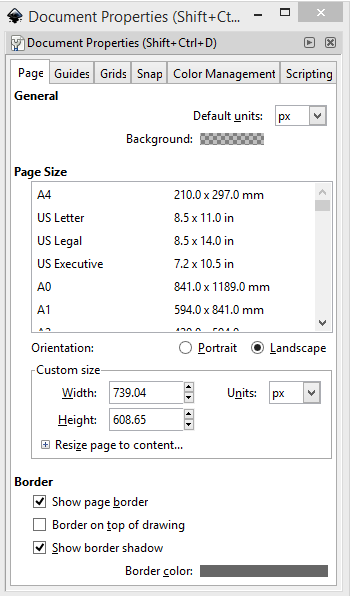
\includegraphics  {obrazky/obr4.png}
		\caption{obrázok 4}
		\label{picture4}
	\end{center}
\end{figure}

Plná nádrž ma nasledovne parametre:

\begin{figure}[ht]
	\begin{center}
		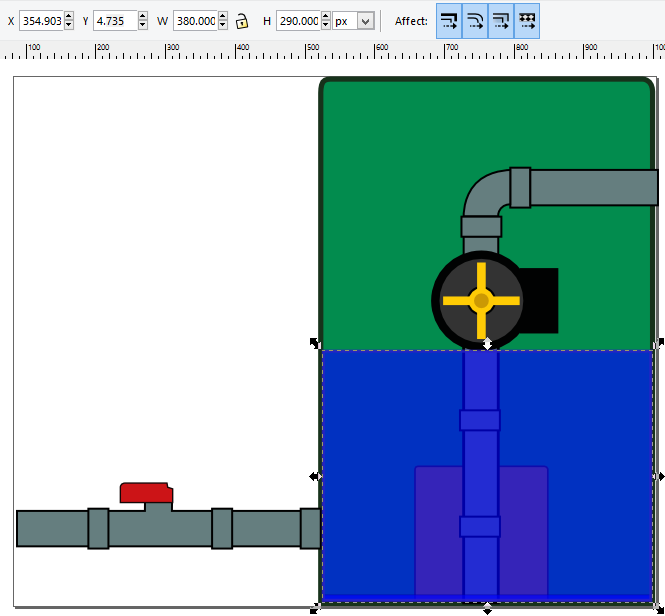
\includegraphics [width=10cm]  {obrazky/obr5.png}
		\caption{obrázok 5}
		\label{picture5}
	\end{center}
\end{figure}

V SVG súbore je to 
\begin{verbatim}

Inkscape:label="\#hladina"
y="1320.1689"
x="2507.8459"
height="605.83868"
width="797.04492"
id="hladina"
\end{verbatim}


Prázdna nádrž
\begin{figure}[ht]
	\begin{center}
		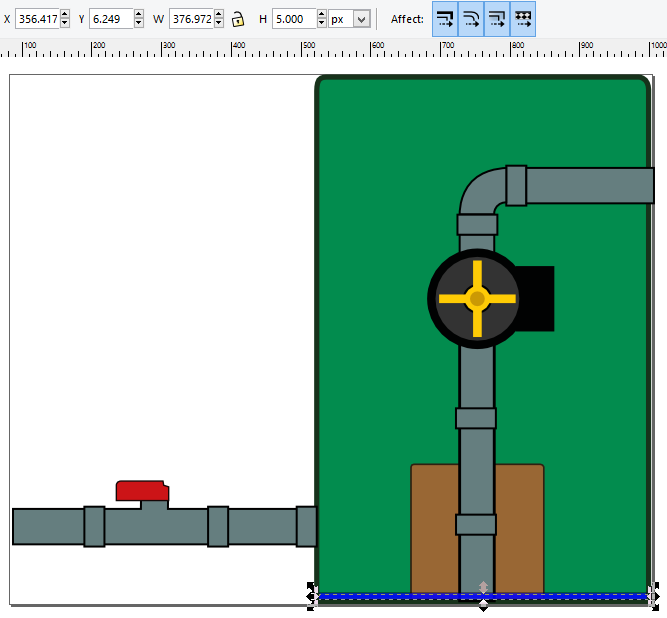
\includegraphics [width=10cm]  {obrazky/obr6.png}
		\caption{obrázok 6}
		\label{picture6}
	\end{center}
\end{figure}

v SVG to je nasledovne 
\begin{lstlisting}[language=html]
<rect
inkscape:label="\#hladina"
y="1916.3605"
x="2507.8459"
height="9.6471272"
width="797.04492"
id="hladina"
...
\end{lstlisting}



Hladina nádrže:
vykreslená ako obdĺžnik
\begin{lstlisting} [language=html]
<rect
	inkscape:label="#hladina"
	y="1320.1689"
	x="2507.8459"
	height="605.83868"
	width="797.04492"
	id="hladina"
	style=
		"fill:#0000ff;
		fill-opacity:0.65098039;
		fill-rule:evenodd;
		stroke:#2c20c8;
		stroke-width:7.42523718px;
		stroke-linecap:butt;
		stroke-linejoin:miter;
		stroke-opacity:0.80952382">
<desc id="desc3119-4">hladina</desc>
<title id="title3117-0">hladina</title>
</rect>
\end{lstlisting}


Parametre ako stroke, fill, a iné sa dajú meniť prostredníctvom attr v Snap. … TODO

